\section{Abstract concepts}

The function of the transport layer is to facilitate exchange of serialized representations of DSDL objects\footnote{%
    DSDL and data serialization are reviewed in chapter~\ref{sec:dsdl}.
} between UAVCAN nodes over the \emph{transport network}.

\subsection{Transport model}\label{sec:transport_model}

This section introduces an abstract implementation-agnostic model of the UAVCAN transport layer.
The core relations are depicted in figure~\ref{fig:transport_model}.
Some of the concepts introduced at this level may not be manifested in the design of concrete transports;
despite that, they are convenient for an abstract discussion.

% Please do not remove the hard placement specifier [H], it is needed to keep elements ordered.
\begin{figure}[H]
    \centering
    \resizebox{\textwidth}{!}{
        \footnotesize
        \begin{tabu}{|l l l|X[c,2] X[c] X[c]|l|}\hline\rowfont{\bfseries}
            \multicolumn{3}{|c|}{Taxonomy} &
            Message transfers &
            \multicolumn{2}{|c|}{Service transfers} &
            Description \\\hline

            % TRANSFER PAYLOAD
            \multicolumn{3}{|c|}{Transfer payload} &
            \multicolumn{3}{c|}{\bfseries{} Serialized object} &
            The serialized instance of a specific DSDL data type. \\\hline

            % TRANSFER PRIORITY
            \multicolumn{1}{|c|}{\multirow{7}{*}{\rotatebox[origin=c]{90}{Transfer metadata}}} &
            &
            &
            \multicolumn{3}{c|}{\bfseries{} Transfer priority} &
            Defines the urgency (time sensitivity) of the transferred object.\\\cline{4-7}

            % TRANSFER ID
            \multicolumn{1}{|c|}{} &
            &
            &
            \multicolumn{3}{c|}{\bfseries{} Transfer-ID} &
            An integer that uniquely identifies a transfer within its session.\\\cline{2-7}

            % ROUTE SPECIFIER
            \multicolumn{1}{|c|}{} &
            \multicolumn{1}{c|}{\multirow{5}{*}{\rotatebox[origin=c]{90}{\shortstack{Session \\ specifier}}}} &
            \multirow{2}{*}{\shortstack{Route \\ specifier}} &
            \multicolumn{3}{c|}{\bfseries{} Source node-ID} &
            Source node-ID is not specified for anonymous transfers. \\\cline{5-6}

            \multicolumn{1}{|c|}{} &
            \multicolumn{1}{c|}{} &
            &
            \multicolumn{1}{c|}{} &
            \multicolumn{2}{c|}{\bfseries{} Destination node-ID} &
            Destination node-ID is not specified for broadcast transfers.\\\cline{3-7}

            % DATA SPECIFIER
            \multicolumn{1}{|c|}{} &
            \multicolumn{1}{c|}{} &
            \multirow{3}{*}{\shortstack{Data \\ specifier}} &
            \multicolumn{1}{c|}{\multirow{2}{*}{\bfseries{} Subject-ID}} &
            \multicolumn{2}{c|}{\bfseries{} Service-ID} &
            Port-ID specifies how the serialized object should be processed.\\\cline{5-6}

            \multicolumn{1}{|c|}{} &
            \multicolumn{1}{c|}{} &
            &
            \multicolumn{1}{c|}{} &
            {\bfseries{} Request} &
            {\bfseries{} Response} &
            Request/response specifier applies to services only.\\\cline{4-6}

            \multicolumn{1}{|c|}{} &
            \multicolumn{1}{c|}{} &
            &
            \multicolumn{3}{c|}{\bfseries{} Transfer kind} &
            Message (subject) or service transfer.\\\hline
        \end{tabu}
    }
    \caption{UAVCAN transport layer model}\label{fig:transport_model}
\end{figure}

\subsubsection{Transfer}

A \emph{transfer} is a singular act of data transmission from one UAVCAN node to zero or more other UAVCAN nodes
over the transport network.
A transfer carries zero or more bytes of \emph{transfer payload} together with the associated \emph{transfer metadata},
which encodes the semantic and temporal properties of the carried payload.
The elements comprising the metadata are reviewed below.

Transfers are distinguished between \emph{message transfers} and \emph{service transfers} depending on the kind
of the carried DSDL object.
Service transfers are further differentiated between \emph{service request transfers},
which are sent from the invoking node -- \emph{client node} -- to the node that provides the service --
\emph{server node}, and \emph{service response transfers},
which are sent from the server node to the client node upon handling the request.

A transfer is manifested on the transport network as one or more \emph{transport frames}.
A transport frame is an atomic entity carrying the entire transfer payload or a fraction thereof
with the associated transfer metadata --
possibly extended with additional elements specific to the concrete transport --
over the transport network.
The exact definition of a transport frame and the mapping of the abstract transport model onto it
are specific to concrete transports\footnote{
    For example, UAVCAN/CAN (introduced later) defines a particular CAN frame format.
    Frames that follow the format are UAVCAN transport frames of UAVCAN/CAN.
}.

\subsubsection{Transfer payload}\label{sec:transport_transfer_payload}

The transfer payload contains the serialized representation of the carried
DSDL object\footnote{Chapter~\ref{sec:dsdl}.}.

Concrete transports may extend the payload with zero-valued \emph{padding bytes} at the end
to meet the transport-specific data granularity constraints.
Usage of non-zero-valued padding bytes is prohibited for all implementations\footnote{%
    Non-zero padding bytes are disallowed because they would interfere with the implicit zero extension rule
    (section~\ref{sec:dsdl_data_serialization}).
}.

Concrete transports may extend the payload with a \emph{transfer CRC}
-- an additional metadata field used for validating its integrity.
The details of its implementation are dictated by the concrete transport specification.

The deterministic nature of UAVCAN in general and DSDL in particular allows implementations to statically determine
the maximum amount of memory that is required to contain the serialized representation
of a DSDL object of a particular type.
Consequently, an implementation that is interested in receiving data objects of a particular type
can statically determine the maximum length of the transfer payload.

Implementations should handle incoming transfers containing a larger amount of payload data than expected.
In the event of such extra payload being received, a compliant implementation should
discard the excessive (unexpected) data at the end of the received payload\footnote{%
    Such occurrence is not indicative of a problem so it should not be reported as such.
}.
The transfer CRC, if applicable, shall be validated regardless of the presence of the extra payload in the transfer.
See figure~\ref{fig:transport_payload_truncation}.

A \emph{transport-layer maximum transmission unit} (MTU) is the maximum amount of data with the associated metadata
that can be transmitted per transport frame for a particular concrete transport.
All nodes connected to a given transport network should share the same transport-layer MTU setting\footnote{%
    Failure to follow this rule may render nodes unable to communicate if a transmitting node emits larger transport
    frames than the receiving node is able to accept.
}.

In order to facilitate the implicit zero extension rule introduced in section~\ref{sec:dsdl_data_serialization},
implementations shall not discard a transfer even if it is determined that it contains less payload
data than a predicted minimum.

A transfer whose payload exceeds the capacity of the transport frame is manifested on the transport network
as a set of multiple transport frames; such transfers are referred to as \emph{multi-frame transfers}.
Implementations shall minimize the number of transport frames constituting a multi-frame transfer by ensuring that
their payload capacity is not underutilized.
Implementations should minimize the delay between transmission of transport frames that belong to the same transfer.
Transport frames of a multi-frame transfer shall be transmitted following the order of the
transfer payload fragments they contain.

A transfer whose payload does not exceed the capacity of the transport frame shall be manifested on the transport
network as a single transport frame\footnote{%
    In other words, multi-frame transfers are prohibited for payloads that can be transferred
    using a single-frame transfer.
}; such transfers are referred to as \emph{single-frame transfers}.

\begin{figure}[H]
    $$
    \raisebox{1em}{\footnotesize{\text{first byte}}}
    \overbrace{%
        \underbrace{%
            \blacksquare\blacksquare\blacksquare\blacksquare\blacksquare\blacksquare%
            \blacksquare\blacksquare\blacksquare\blacksquare\blacksquare\blacksquare%
        }_{\substack{\text{Expected, accepted} \\ \text{payload}}}%
        \underbrace{%
            \boxtimes\boxtimes\boxtimes\boxtimes\boxtimes\boxtimes\boxtimes\boxtimes%
        }_{\substack{\text{Excessive, discarded} \\ \text{payload}}}%
    }^{\substack{%
        \text{Transfer CRC is validated} \\
        \text{for the entire transfer payload} \\
        \text{before the truncation}}
    }
    \raisebox{1em}{\footnotesize{\text{last byte}}}
    $$
    \caption{Transfer payload truncation\label{fig:transport_payload_truncation}}
\end{figure}

\begin{remark}[breakable]
    The requirement to discard the excessive payload data at the end of the transfer is motivated by
    the necessity to allow extensibility of data type definitions, as described in chapter~\ref{sec:dsdl}.
    Additionally, excessive payload data may contain zero padding bytes if required by the concrete transport.

    Let node $A$ publish an object of the following type over the subject $x$:

    \begin{minted}{python}
        float32 parameter
        float32 variance
    \end{minted}

    Let node $B$ subscribe to the subject $x$ expecting an object of the following type:

    \begin{minted}{python}
        float32 parameter
    \end{minted}

    The payload truncation requirement guarantees that the two nodes will be able to interoperate despite
    relying on incompatible data type definitions.
    Under this example, the duty of ensuring the semantic compatibility lies on the system integrator.

    The requirement that all involved nodes use the same transport-layer MTU is crucial here.
    Suppose that the MTU expected by the node $B$ is four bytes and the MTU of the node $A$ is eight bytes.
    Under this setup, messages emitted by $A$ would be contained in single-frame transfers that are too large
    for $B$ to process, resulting in the nodes being unable to communicate.
    An attempt to optimize the memory utilization of $B$ by relying on the fact that the maximum length of a
    serialized representation of the message is four bytes would be a mistake, because this assumption ignores
    the existence of subtyping and introduces leaky abstractions throughout the protocol stack.
\end{remark}

\begin{remark}[breakable]
    The implicit zero extension rule makes deserialization routines sensitive to the trailing unused data.
    For example, suppose that a publisher emits an object of type:

    \begin{minted}{python}
        uint16 foo
    \end{minted}

    Suppose that the concrete transport at hand requires padding to 4 bytes, which is done with $55_{16}$
    (intentionally non-compliant for the sake of this example).
    Suppose that the published value is $1234_{16}$,
    so the resulting serialized representation is $\left[34_{16}, 12_{16}, 55_{16}, 55_{16}\right]$.
    Suppose that the receiving side relies on the implicit zero extension rule with the following definition:

    \begin{minted}{python}
        uint16 foo
        uint16 bar
    \end{minted}

    The expectation is that \verb|foo| will be deserialized as $1234_{16}$,
    and \verb|bar| will be zero-extended as $0000_{16}$.
    If arbitrary padding values were allowed, the value of \verb|bar| would become undefined;
    in this particular example it would be $5555_{16}$.

    Therefore, the implicit zero-extension rule requires that padding is done with zero bytes only.
\end{remark}

\subsubsection{Transfer priority}\label{sec:transport_transfer_priority}

Transfers are prioritized by means of the \emph{transfer priority} parameter,
which allows at least 8 (eight) distinct priority levels.
Concrete transports may support more than eight priority levels.

Transmission of transport frames shall be ordered so that frames of higher priority are transmitted first.
It follows that higher-priority transfers may preempt transmission of lower-priority transfers.

Transmission of transport frames that share the same priority level should follow the order of their appearance in
the transmission queue.

Priority of message transfers and service request transfers can be chosen freely
according to the requirements of the application.
Priority of a service response transfer should match the priority of the corresponding service request transfer.

\begin{remark}[breakable]
    Transfer prioritization is paramount for distributed real-time applications.

    The priority level mnemonics and their usage recommendations are specified in the following list.
    The mapping between the mnemonics and actual numeric identifiers is transport-dependent.

    % https://forum.uavcan.org/t/transfer-priority-level-mnemonics/218/6?u=pavel.kirienko
    \begin{description}
        \item[Exceptional] -- The bus designer can ignore these messages when calculating bus load since they
        should only be sent when a total system failure has occurred.
        For example, a self-destruct message on a rocket would use this priority.
        Another analogy is an NMI on a microcontroller.

        \item[Immediate] -- Immediate is a ``high priority message'' but with additional latency constraints.
        Since exceptional messages are not considered when designing a bus, the latency of immediate messages
        can be determined by considering only immediate messages.

        \item[Fast] -- Fast and immediate are both ``high priority messages'' but with additional latency constraints.
        Since exceptional messages are not considered when designing a bus,
        the latency of fast messages can be determined by considering only immediate and fast messages.

        \item[High] -- High priority messages are more important than nominal messages but have looser
        latency requirements than fast messages. This priority is used so that,
        in the presence of rogue nominal messages, important commands can be received.
        For example, one might envision a failure mode where a temperature sensor starts to
        load a vehicle bus with nominal messages.
        The vehicle remains operational (for a time) because the controller is exchanging fast and
        immediate messages with sensors and actuators.
        A system safety monitor is able to detect the distressed bus and command the vehicle to a
        safe state by sending high priority messages to the controller.

        \item[Nominal] -- This is what all messages should use by default.
        Specifically the heartbeat messages should use this priority.

        \item[Low] -- Low priority messages are expected to be sent on a bus under all conditions but cannot
        prevent the delivery of nominal messages.
        They are allowed to be delayed but latency should be constrained by the bus designer.

        \item[Slow] -- Slow messages are low priority messages that have no time sensitivity at all.
        The bus designer need only ensure that, for all possible system states,
        these messages will eventually be sent.

        \item[Optional] -- These messages might never be sent (theoretically) for some possible system states.
        The system shall tolerate never exchanging optional messages in every possible state.
        The bus designer can ignore these messages when calculating bus load.
        This should be the priority used for diagnostic or debug messages that are not required on an
        operational system.
    \end{description}
\end{remark}

\subsubsection{Route specifier}\label{sec:transport_route_specifier}

The \emph{route specifier} defines the node-ID of the origin and the node-ID of the destination of a transfer.

A \emph{broadcast transfer} is a transfer that does not have a specific destination;
the decision of whether to process a broadcast transfer is delegated to receiving nodes\footnote{%
    This does not imply that applications are required to be involved with every broadcast transfer.
    The opt-in logic is facilitated by the low-level routing and/or filtering features implemented
    by the network stack and/or the underlying hardware.
}.
A \emph{unicast transfer} is a transfer that is addressed to a specific single node\footnote{%
    Whose existence and availability is optional.
} whose node-ID is not the same as that of the origin;
which node should process a unicast transfer is decided by the sending node.

A node that does not have a node-ID is referred to as \emph{anonymous node}.
Such nodes are unable to emit transfers other than \emph{anonymous transfers}.
An anonymous transfer is a transfer that does not have a specific source.
Anonymous transfers have the following limitations\footnote{%
    Anonymous transfers are intended primarily for the facilitation of the optional plug-and-play feature
    (section~\ref{sec:application_functions})
    which enables fully automatic configuration of UAVCAN nodes upon their connection to the network.
    Some transports may provide native support for auto-configuration, rendering anonymous transfers unnecessary.
}:
\begin{itemize}
    \item An anonymous transfer can be only a message transfer.
    \item An anonymous transfer can be only a single-frame transfer.
    \item Concrete transports may introduce arbitrary additional restrictions
          on anonymous transfers or omit their support completely.
\end{itemize}

A message transfer can be only a broadcast transfer; unicast message transfers are not defined\footnote{%
    Unicast message transfers may be defined in a future revision of this Specification.
}.
A service transfer can be only a unicast transfer; broadcast service transfers are prohibited.

\begin{UAVCANCompactTable}{|l l l|}
    Transfer kind       & Unicast       & Broadcast     \\
    Message transfer    & Not defined   & Valid         \\
    Service transfer    & Valid         & Prohibited    \\
\end{UAVCANCompactTable}

\subsubsection{Data specifier}\label{sec:transport_data_specifier}

The \emph{data specifier} encodes the semantic properties of the DSDL object carried by a transfer and its kind.

The data specifier of a message transfer is the subject-ID of the contained DSDL message object.

The data specifier of a service transfer is a combination of the service-ID of the contained DSDL service object
and an additional binary parameter that segregates service requests from service responses.

\subsubsection{Session specifier}\label{sec:transport_session_specifier}

The \emph{session specifier} is a combination of the data specifier and the route specifier.
Its function is to uniquely identify a category of transfers by the semantics of exchanged data and
the agents participating in its exchange while abstracting over individual transfers and their concrete data\footnote{%
    Due to the fact that anonymous transfers lack information about their origin,
    all anonymous transfers that share the same data specifier and destination
    are grouped under the same session specifier.
}.

The term \emph{session} used here denotes the node's local representation of a logical communication
channel that it is a member of.
Following the stateless and low-context nature of UAVCAN, this concept excludes any notion of explicit state sharing
between nodes.

\begin{remark}[breakable]
    One of the key design principles is that UAVCAN is a stateless low-context protocol where collaborating agents
    do not make strong assumptions about the state of each other.
    Statelessness and context invariance are important because they facilitate behavioral simplicity and robustness;
    these properties are desirable for deterministic real-time distributed applications which UAVCAN is designed for.

    Design and verification of a system that relies on multiple agents sharing the same model of a distributed process
    necessitates careful analysis of special cases such as unintended state divergence, latency and transient states,
    sudden loss of state (e.g., due to disconnection or a software reset), etc.
    Lack of adequate consideration may render the resulting solution fragile and prone to unspecified behaviors.

    Some of the practical consequences of the low-context design include the ability of a node to immediately
    commence operation on the network without any prior initialization steps.
    Likewise, addition and removal of a subscriber to a given subject is transparent to the publisher.

    The above considerations only hold for the communication protocol itself.
    Applications whose functionality is built on top of the protocol may engage in state sharing if such is
    found to be beneficial\footnote{%
        Related discussion in
        \url{https://forum.uavcan.org/t/idempotent-interfaces-and-deterministic-data-loss-mitigation/643}.
    }.
\end{remark}

\begin{remark}[breakable]
    Some implementations of the UAVCAN communication stack may contain states indexed by the session specifier.
    For example, in order to emit a transfer, the stack may need to query the appropriate transfer-ID counter
    (section~\ref{sec:transport_transfer_id}) by the session specifier of the transfer.
    Likewise, in order to process a received frame,
    the stack may need to locate the appropriate states keyed by the session specifier.

    Given the intended application domains of UAVCAN,
    the temporal characteristics of such look-up activities should be well-characterized and predictable.
    Due to the fact that all underlying primitive parameters that form the session specifier
    (such as node-ID, port-ID, etc.) have statically defined bounds,
    it is trivial to construct a look-up procedure satisfying any computational complexity envelope,
    from constant-complexity $O(1)$ at the expense of heightened memory utilization,
    up to low-memory-footprint $O(n)$ if temporal predictability is less relevant.

    For example, given a subject-ID, the maximum number of distinct sessions that can be observed
    by the local node will never exceed the number of nodes in the network minus one\footnote{%
        A node cannot receive transfers from itself, hence minus one.
    }.
    If the number of nodes in the network cannot be reliably known in advance (which is the case in most applications),
    it can be considered to equal the maximum number of nodes permitted by the concrete transport\footnote{%
        E.g., 128 nodes for the CAN bus transport.
    }.
    The total number of distinct sessions that can be observed by a node is a product of the number
    of distinct data specifiers utilized by the node and the number of other nodes in the network.

    It is recognized that highly rigid safety-critical applications may benefit from avoiding any
    dynamic look-up by sacrificing generality, by employing automatic code generation, or through other methods,
    in the interest of greater determinism and robustness.
    In such cases, the above considerations may be irrelevant.
\end{remark}

\subsubsection{Transfer-ID}\label{sec:transport_transfer_id}

The \emph{transfer-ID} is an unsigned integer value that is provided for every transfer.
Barring the case of transfer-ID overflow reviewed below,
each transfer under a given session specifier has a unique transfer-ID value.
This parameter is crucial for many aspects of UAVCAN communication\footnote{%
    One might be tempted to use the transfer-ID value for temporal synchronization of
    parallel message streams originating from the same node,
    where messages bearing the same transfer-ID value are supposed to correspond to the same moment in time.
    Such use is strongly discouraged because it is incompatible with transports that rely on overflowing
    transfer-ID values and because it introduces a leaky abstraction into the system.
    If temporal synchronization is necessary, explicit time stamping should be used instead.
}; specifically:

\begin{description}
    \item[Message sequence monitoring] -- transfer-ID allows receiving nodes to detect discontinuities
    in incoming message streams from remote nodes.

    \item[Service response matching] -- when a server responds to a request, it uses the same transfer-ID for the
    response transfer as in the request transfer,
    allowing the client to emit concurrent requests to the same server while being able to
    match each response with the corresponding local request state.

    \item[Transfer deduplication] -- the transfer-ID allows receiving nodes to detect and eliminate duplicated
    transfers.
    Transfer duplication may occur either spuriously as an artifact of a concrete transport\footnote{%
        For example, in CAN bus, a frame that appears valid to the receiver may under certain (rare) conditions
        appear invalid to the transmitter, triggering the latter to retransmit the frame,
        in which case it will be duplicated on the side of the receiver.
        Sequence counting mechanisms such as transfer-ID allow implementations to circumvent this problem.
    } or deliberately as a method of deterministic data loss mitigation for unreliable links
    (section~\ref{sec:transport_deterministic_data_loss_mitigation}).

    \item[Multi-frame transfer reassembly] -- a transfer that is split over multiple transport frames is reassembled
    back upon reception with the help of transfer-ID: all transport frames that comprise a transfer
    share the same transfer-ID value.

    \item[Automatic management of redundant interfaces] -- in redundant transport networks,
    transfer-ID enables automatic switchover to a back-up interface shall the primary interface fail.
    The switchover logic can be completely transparent to the application, joining several independent
    redundant transport networks into a highly reliable single virtual communication channel.
\end{description}

For service response transfers the transfer-ID value shall be directly copied from the corresponding
service request transfer\footnote{This behavior facilitates request-response matching on the client node.}.

A node that is interested in emitting message transfers or service request transfers
under a particular session specifier, whether periodically or on an ad-hoc basis,
shall allocate a transfer-ID counter state associated with said session specifier exclusively.
The transfer-ID value of every emitted transfer is determined by sampling the corresponding counter
keyed by the session specifier of the transfer; afterwards, the counter is incremented by one.

The initial value of a transfer-ID counter shall be zero.
Once a new transfer-ID counter is created,
it shall be kept at least as long as the node remains connected to the transport network;
destruction of transfer-ID counter states is prohibited\footnote{%
    The number of unique session specifiers is bounded and can be determined statically per application,
    so this requirement does not introduce non-deterministic features into the application even if it leverages
    aperiodic/ad-hoc transfers.
}.

When the transfer-ID counter reaches the maximum value defined for the concrete transport,
the next increment resets its value to zero.
Transports where such events are expected to take place during operation are said to have \emph{cyclic transfer-ID};
the number of unique transfer-ID values is referred to as \emph{transfer-ID modulo}.
Transports where the maximum value of the transfer-ID is high enough to be unreachable under all conceivable
practical circumstances are said to have \emph{monotonic transfer-ID}.

\emph{Transfer-ID difference} for a pair of transfer-ID values $a$ and $b$ is defined
for monotonic transfer-ID as their arithmetic difference $a-b$.
For a cyclic transfer-ID, the difference is defined as the number of increment operations that need to be applied
to $b$ so that $a = b^\prime{}$.

\begin{remark}
    A C++ implementation of the cyclic transfer-ID difference operator is provided here.
    \begin{minted}{cpp}
        #include <cstdint>
        /**
         * UAVCAN cyclic transfer-ID difference computation algorithm implemented in C++.
         * License: CC0, no copyright reserved.
         * @param a         Left-hand operand (minuend).
         * @param b         Right-hand operand (subtrahend).
         * @param modulo    The number of distinct transfer-ID values, or the maximum value plus one.
         * @returns         The number of increment operations separating b from a.
         */
        [[nodiscard]]
        constexpr std::uint8_t computeCyclicTransferIDDifference(const std::uint8_t a,
                                                                 const std::uint8_t b,
                                                                 const std::uint8_t modulo)
        {
            std::int16_t d = static_cast<std::int16_t>(a) - static_cast<std::int16_t>(b);
            if (d < 0)
            {
                d += static_cast<std::int16_t>(modulo);
            }
            return static_cast<std::uint8_t>(d);
        }
    \end{minted}
\end{remark}

\subsection{Redundant transports}

UAVCAN supports transport redundancy for the benefit of a certain class of safety-critical applications.
A redundant transport interconnects nodes belonging to the same network (all or their subset)
via more than one transport network.
A set of such transport networks that together form a redundant transport is referred to as a
\emph{redundant transport group}.

Each member of a redundant transport group shall be capable of independent operation
such that the level of service of the resulting redundant transport remains constant
as long as at least one member of the redundant group remains functional\footnote{%
    Redundant transports are designed for increased fault tolerance, not for load sharing.
}.

\begin{remark}
    Networks containing nodes with different reliability requirements may benefit from
    nonuniform redundant transport configurations, where non-critical nodes are interconnected
    using a lower number of transports than critical nodes.

    Designers should recognize that nonuniform redundancy may complicate the analysis of the network.
\end{remark}

% The following fragment deals with heterogeneous transports.
% Its inclusion in the body of the document does not make sense until the UDP/IP and Serial transports
% (and/or other transports) are formally specified. When they are, this fragment will be uncommented.
\begin{comment}
\subsubsection{Heterogeneous redundant transports}

A \emph{heterogeneous redundant transport} is a redundant transport configuration where nodes are
interconnected using different concrete transports.
Heterogeneous transports may facilitate higher fault tolerance provided that the failure modes of involved transports
are sufficiently dissimilar\footnote{%
    Consider a heterogeneous configuration combining wired and wireless transports.
    See also ``Wireless Avionics Intra-Communications'' (WAIC).
}.
A heterogeneous redundant transport shall meet \emph{either} of the following requirements:
\begin{itemize}
    \item All of the involved transports shall use monotonic transfer-ID\footnote{%
              Section~\ref{sec:transport_transfer_id}.
          }.
          In this case, the resulting redundant transport is said to be a monotonic transfer-ID transport as well.

    \item All of the involved transports shall use cyclic transfer-ID with identical value ranges.
          In this case, the resulting redundant transport is said to be a cyclic transfer-ID transport as well.
\end{itemize}

\begin{remark}[breakable]
    Transports with monotonic transfer-ID have a higher metadata overhead per frame due to the requirement
    to accommodate a sufficiently wide integer field for the transfer-ID value.
    Their advantage is that transfer-ID values of all transports in a redundant group
    are guaranteed to remain in-phase as long as the node is running.
    The importance of this guarantee can be demonstrated with the following counterexample
    of two transports leveraging different transfer-ID ranges for the same session,
    where the unambiguous mapping between their transfer-ID values is lost after the first overflow
    (figure~\ref{fig:transport_cyclic_transfer_id_redundant}).

    % Plot[{
    %   Mod[x, 40],
    %   Mod[x, 32]
    %  },
    %  {x, 0, 150},
    %  PlotLegends -> {"[0,40]", "[0,32]"},
    %  GridLines -> {{}, {32, 40}},
    %  AxesLabel -> {"Count", "Transfer-ID"},
    %  Epilog -> {
    %    Text["Epoch 0", {20, 35}],
    %    Text["Epoch 1", {60, 35}],
    %    Text["Epoch 2", {100, 35}],
    %    Text["Epoch 3", {140, 35}]
    %   }
    %  ]
    \begin{figure}[H]
        \centering
        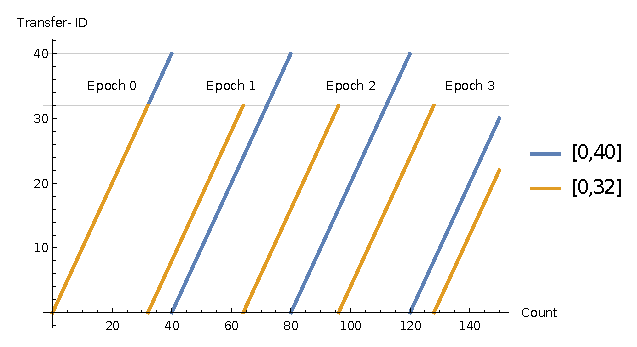
\includegraphics[width=0.6\textwidth]{transport/cyclic_transfer_id_redundant_transport}
        \caption{Issues with cyclic transfer-ID in heterogeneous redundant transports}
        \label{fig:transport_cyclic_transfer_id_redundant}
    \end{figure}
\end{remark}
\end{comment}

\subsection{Transfer transmission}

\subsubsection{Transmission timeout}

The transport frames of a time-sensitive transfer whose payload has lost relevance due to
its transmission being delayed should be removed from the transmission queue\footnote{%
    Trailing transport frames of partially transmitted multi-frame transfers should be removed as well.
    The objective of this recommendation is to ensure that obsolete data is not transmitted
    as it may have adverse effects on the system.
}.
The time interval between the point where the transfer is constructed and the point where it is considered
to have lost relevance is referred to as \emph{transmission timeout}.

% "Output port" sounds better but this term is not defined.
The transmission timeout should be documented for each outgoing transfer port.

\subsubsection{Pending service requests}

In the case of cyclic transfer-ID transports (section~\ref{sec:transport_transfer_id}),
implementations should ensure that upon a transfer-ID overflow a service client session
does not reuse the same transfer-ID value for more than one pending request simultaneously.

\subsubsection{Deterministic data loss mitigation}\label{sec:transport_deterministic_data_loss_mitigation}

Performance of transport networks where the probability of a successful transfer delivery
does not meet design requirements can be adjusted by repeating relevant outgoing transfers
under the same transfer-ID value\footnote{%
    Removal of intentionally duplicated transfers on the receiving side is natively guaranteed
    by this transport layer specification;
    no special activities are needed there to accommodate this feature.
}.
This tactic is referred to as \emph{deterministic data loss mitigation}\footnote{%
    Discussed in
    \url{https://forum.uavcan.org/t/idempotent-interfaces-and-deterministic-data-loss-mitigation/643}.
}.

\subsubsection{Transmission over redundant transports}

Nodes equipped with redundant transports shall submit every outgoing transfer to the transmission queues of all
available redundant transports simultaneously\footnote{%
    The objective of this requirement is to guarantee that a redundant transport remains fully functional
    as long as at least one transport in the redundant group is functional.
}.
It is recognized that perfectly simultaneous transmission may not be possible due to different
utilization rates of the redundant transports, different phasing of their traffic, and/or application constraints,
in which case implementations should strive to minimize the temporal skew as long as that
does not increase the latency.

An exception to the above rule applies if the payload of the transfer is a function of
the identity of the transport instance that carries the transfer\footnote{%
    An example of such a special case is the time synchronization algorithm documented
    in section~\ref{sec:application_functions}.
}.

\subsection{Transfer reception}\label{sec:transport_transfer_reception}

\subsubsection{Definitions}

\emph{Transfer reassembly} is the real-time process of reconstruction of the transfer payload and its metadata from
a sequence of relevant transport frames.

\emph{Transfer-ID timeout} is a time interval whose semantics are explained below.
Implementations may define this value statically according to the application requirements.
Implementations may automatically adjust this value per session at runtime as a function of the
observed transfer reception interval.
Transfer-ID timeout values greater than 2 (two) seconds are not recommended.
Implementations should document the value of transfer-ID timeout or the rules of its computation.

\emph{Transport frame reception timestamp} specifies the moment of time when the frame is received by a node.
\emph{Transfer reception timestamp} is the reception timestamp of the earliest received frame of the transfer.

An \emph{ordered transfer sequence} is a sequence of transfers whose temporal order is
covariant with their transfer-ID values.

\subsubsection{Behaviors}

For a given session specifier, every unique transfer
(differentiated from other transfers in the same session by its transfer-ID)
shall be received at most once\footnote{%
    In other words, intentional and unintentional duplicates shall be removed.
    Intentional duplications are introduced by the deterministic data loss mitigation measure or redundant transports.
    Unintentional duplications may be introduced by various artifacts of the transport network.
}.

For a given session specifier, a successfully reassembled transfer that is temporally separated from
any other successfully reassembled transfer under the same session specifier by more than the transfer-ID timeout
is considered unique regardless of its transfer-ID value.

If the optimal transfer-ID timeout value for a given session cannot be known in advance,
it can be computed at runtime on a per-session basis\footnote{%
    E.g., as a multiple of the average transfer reception interval.
}.
The parameters of such computation are to be chosen according to the requirements of the application,
but they should always be documented.

\begin{remark}
    Low transfer-ID timeout values increase the risk of undetected transfer duplication when such transfers
    are significantly delayed due to network congestion,
    which is possible with very low-priority transfers when the network load is high.

    High transfer-ID timeout values increase the risk of an undetected transfer loss
    when a remote node suffers a loss of state (e.g., due to a software reset).

    The ability to auto-detect the optimal transfer-ID timeout value per session at runtime ensures that the
    application can find the optimal balance even if the temporal properties of the network are not known in advance.
    As a practical example, an implementation could compute the exponential moving average of the
    transfer reception interval $x$ for a given session and define the transfer-ID timeout as $2x$.

    It is important to note that the automatic adjustment of the transfer-ID timeout should only be done
    on a per-session basis rather than for the entire port, because there may be multiple remote nodes
    emitting transfers on the same port at different rates.
    For example, if one node emits transfers at a rate $r$ transfers per second, and another node emits transfers
    on the same port at a much higher rate $100r$, the resulting auto-detected transfer-ID timeout might be
    too low, creating the risk of accepting duplicates.
\end{remark}

Implementations are recommended, but not required, to support reassembly of
multi-frame transfers where the temporal ordering of the transport frames is distorted.

\begin{remark}
    For a certain category of transport implementations, reassembly of multi-frame transfers from an
    unordered transport frame sequence increases the probability of successful delivery if
    the probability of a transport frame loss is non-zero and transport frames are intentionally duplicated.

    Such intentional duplication occurs in redundant transports and if deterministic data loss mitigation is used.
    The reason is that the loss of a single transport frame is observed by the receiving node as its relocation
    from its original position in the sequence to the position of its duplicate.
\end{remark}

Reassembled transfers shall form an ordered transfer sequence.

For a cyclic transfer-ID redundant transport whose redundant group contains $n$ transports,
if up to $n-1$ transports in the redundant group lose the ability to exchange transport frames between nodes,
the transfer reassembly process shall be able to restore nominal functionality
in an amount of time that does not exceed the transfer-ID timeout.

\begin{remark}
    Cyclic transfer-ID transport implementations are recommended to insert a delay before performing
    an automatic fail-over.
    As indicated in the normative description, the delay may be arbitrary as long as it does not exceed the
    transfer-ID timeout value.

    The fail-over delay allows implementations to uphold the transfer uniqueness requirement when the phasing of
    traffic on different transports within the redundant group differs by more than the transfer-ID overflow period.
\end{remark}

For a monotonic transfer-ID redundant transport whose redundant group contains $n$ transports,
if up to $n-1$ transports in the redundant group lose the ability to exchange transport frames between nodes,
the performance of the transfer reassembly process shall not be affected.

\begin{remark}
    Monotonic transfer-ID transport implementations are recommended to always accept the first transfer
    to arrive regardless of which transport within the redundant group it was delivered over.

    This behavior ensures that the total latency of a redundant transport equals the latency of the best-performing
    transport within the redundant group (i.e., the total latency equals the latency of the fastest transport).
    Since a monotonic transfer-ID does not overflow, there is no risk of failing to uphold the uniqueness guarantee
    unlike with the case of cyclic transfer-ID.
\end{remark}

If anonymous transfers are supported by the concrete transport,
reassembly of anonymous transfers shall be implemented by unconditional acceptance of their transport frames.
Requirements pertaining to ordering and uniqueness do not apply.

\begin{remark}
    Regardless of the concrete transport in use and its capabilities,
    UAVCAN provides the following guarantees (excluding anonymous transfers):

    \begin{itemize}
        \item Removal of duplicates. If a transfer is delivered, it is guaranteed that it is delivered once,
              even if intentionally duplicated by the origin.
        \item Correct ordering. Received transfers are ordered according to their transfer-ID values.
        \item Deterministic automatic fail-over in the event of a failure of a transport (or several)
              in a redundant group.
    \end{itemize}

    For anonymous transfers, ordering and uniqueness are impossible to enforce
    because anonymous transfers that originate from different nodes may share the same session specifier.

    Reassembly of transfers from redundant interfaces may be implemented either on the per-transport-frame level
    or on the per-transfer level.
    The former amounts to receiving individual transport frames from redundant interfaces
    which are then used for reassembly; it can be seen that this method requires that all transports in the
    redundant group use identical application-level MTU (i.e., same number of transfer payload bytes per frame).
    The latter can be implemented by treating each transport in the redundant group separately,
    so that each runs an independent transfer reassembly process, whose outputs are then deduplicated
    on the per-transfer level; this method may be more computationally complex but it provides greater flexibility.
    A detailed discussion is omitted because it is outside of the scope of this specification.
\end{remark}
